\begin{titlepage}

  % AUTH Logo
  \begin{minipage}{0.3\textwidth}
    \begin{flushleft}
      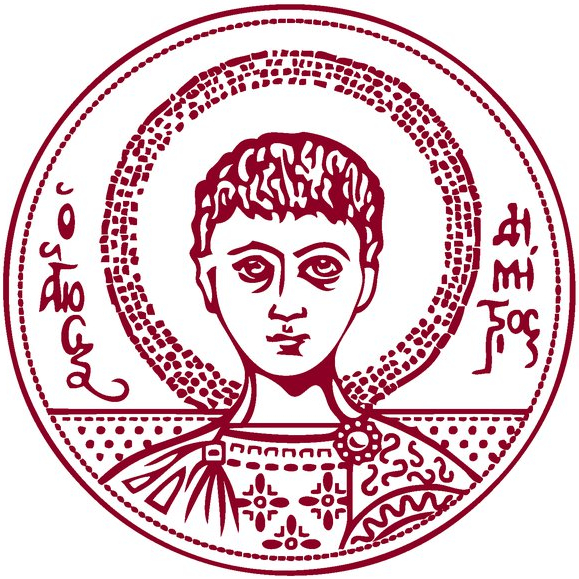
\includegraphics[scale=0.25]{./images/title/authLogoTr.jpg}
    \end{flushleft}
  \end{minipage}
  \begin{minipage}{0.9\textwidth}
    \begin{flushleft}
      \large Αριστοτέλειο Πανεπιστήμιο Θεσσαλονίκης \\
      Πολυτεχνική Σχολή \\
      Τμήμα Ηλεκτρολόγων Μηχανικών $\&$ \\ Μηχανικών Υπολογιστών\\
      
      \normalsize{Τομέας Ηλεκτρονικής και Υπολογιστών} \\
      \normalsize{Εργαστήριο Ευφυών Συστημάτων και Τεχνολογίας\\
      Λογισμικού (ISSEL)} \\[5cm]
    \end{flushleft}
  \end{minipage} \\[1.7cm]




  \begin{center}
    \Large Διπλωματική Εργασία \\[0.8cm]

    \rule{450pt}{4pt} \\[0.4cm]
    {\fontsize{20.26pt}{1em}\selectfont Μοντελοστρεφής ανάπτυξη λογισμικού για IoT συσκευές πραγματικού χρόνου και χαμηλής κατανάλωσης}

    \rule{350pt}{4pt} \\[4cm]

    % Writer
    \begin{minipage}{0.4\textwidth}
      \begin{flushleft} \large
        \emph{Εκπόνηση:} \\
        Αθανάσιος Μανώλης\\
        ΑΕΜ: 8856
      \end{flushleft}
    \end{minipage}
    % Supervisors
    \begin{minipage}{0.45\textwidth}
      \begin{flushright} \large
        \emph{Επίβλεψη:} \\
        Αναπληρωτής Καθηγητής Ανδρέας Λ. Συμεωνίδης\\ 
        Υποψήφιος Διδάκτορας Κωνσταντίνος Παναγιώτου
      \end{flushright}
    \end{minipage}
    \\[1cm]
    \vfill

    % Title
    \large Θεσσαλονίκη, Σεπτέμβριος 2021

  \end{center}
\end{titlepage}
